\section{Sea Ice}
\subsection{Calculation of sea ice melting separately for bare/snow covered ice and meltponds}
Bare ice or snow covered ice: The melt rate is calculated from the net surface heat flux over
ice and the conductive heat flux, with the net surface solar radiation prescribed for bare/snow
covered ice using the respective surface albedo (palsobs). The ice temperature for this part
of the grid box is given by
\begin{align}
T_{i,bare}^{n+1}&=\frac{ H_{Bare} + \frac{C_i}{\Delta t} T_{i,bare}^n +\frac{\kappa_i}{h_{\text{i,eff}}} T_0 } {\frac{C_i}{\Delta t}+\frac{\kappa_i}{h_{\text{i,eff}}} } \label{sea_ice_1}\\
\nonumber \\
\text{where}&\nonumber\\
\nonumber \\
C_i & = \text{heat capacity of the surface ice layer (currently 5 cm)} \nonumber \\
\nonumber \\
\Delta t &= \text{time step}\nonumber \\
\nonumber \\
h_{\text{i,eff}}^n & = h_i^n+\left (\frac {\kappa_i \rho_w}{\kappa_s \rho_s}\right )h_s^n =\text{effective thickness of the ice/snow layer} \nonumber \\
\nonumber \\
h_i^n & = \text{thickness of sea ice at the previous time step}\nonumber \\
\nonumber \\
h_s^n & = \text{thickness of snow (water equivalent) at the previous time step}\nonumber \\
\nonumber \\
\kappa_s & = \text{thermal conductivity of snow} \nonumber \\
\nonumber \\
\kappa_i & = \text{thermal conductivity of ice} \nonumber \\
\nonumber \\
\rho_w, \rho_i & =\text{density of water, ice}  \nonumber \\
\nonumber \\
H_{bare} & = \text{net heat flux over bare/snow covered ice using the respective surface albedo} \nonumber \\
\nonumber \\
T_{i,bare}^n & = \text{ice temperature at the previous time step}  \nonumber \\
\nonumber \\
T_0 & = \text{water temperature below the ice (-1.8°C for ocean)} \nonumber
\end{align}
%
%
%
%
Melting of sea ice over the \underline{bare-ice} fraction of the grid-box can be estimated from
\begin{align}
F_{melt,b}=\left (T_i^{\ast}-T_{melt} \right) \times \left ( \frac{C_i}{\Delta t} + \frac{\kappa_i}{h_{i,eff}^n} \right ) \label{sea_ice_2}> 0
\end{align}
for $T_i^{\ast}>T_{melt}$ , where $T_i^{\ast} = T_{i,bare}^{n+1}$ is the ice temperature at the surface given by (\eqref{sea_ice_1}) and $T_{melt}$ is
the temperature at the melting point (273.15 K). By using (\eqref{sea_ice_1}) in (\eqref{sea_ice_2}), the melt rate can be
written as
\begin{align}
F_{melt,b}=\frac{C_i}{\Delta t}\left (T_{i,bare}^{n}-T_{melt} \right)+H_{bare}-\frac{\kappa_i}{h_{i,eff}^n} \left (T_{melt}-T_{0} \right) \label{sea_ice_3}
\end{align}
If $T_{i,bare}^{n}$ is already at the melting point, the first term vanishes. The melt rate is then given by
the net heat flux $H_{bare}$ minus the conductive heat flux which is positive (downward) for
melting sea ice because $T_{melt}>T_{0}$ . For lake ice, this term vanishes during the melting period.
If $T_{i,bare}^{n}$ is still below the melting point, part of the excess heat $F_{melt,b} > 0$ is used to increase
the ice temperature up to the melting point.

\vspace{2cm}
\noindent{\bf Open melt ponds}: Same as above, but the net surface heat flux $H_{pond}$ is now calculated for
water conditions, using the melt pond albedo for deriving the net surface solar radiation. The
ice temperature below the pond can then be written as
\begin{equation}
T_{i,pond}^{n+1}=\frac{ H_{pond} + \frac{C_i}{\Delta t} T_{i,pond}^n +\frac{\kappa_i}{\left (h_{i}^n-h_{p}^n \right )} T_0 } {\frac{C_i}{\Delta t}+\frac{\kappa_i}{\left (h_i^n-h_p^n \right )} } \label{sea_ice_4}
\end{equation}
where $h_p$ = \underline{local} pond depth = grid-mean pond depth divided by the melt pond fraction $f_p$.
Generally, when the pond is open, $T_{i,pond}^n = T_{melt}$ , but T$_{i,pond}^n < T_{melt}$ just before the melt pond is
formed. In this case, $T_{i,pond}^n$ is set to $T_{i,bare}^n$. The melt rate is given analogously to (\eqref{sea_ice_2}):
\begin{equation}
F_{melt,p}=\left (T_{i}^{\star}-T_{melt} \right)\times \left ( \frac{C_i}{\Delta t} + \frac{\kappa_i}{\left(h_i^n-h_p^n \right)} \right )>0  \label{sea_ice_5}
\end{equation}
for $T_i^{\star}>T_{melt}$ , where $ T_i^{\star} = T_{i,pond}^{n+1}$ is the ice temperature below the pond given by (\eqref{sea_ice_4}). Using
(\eqref{sea_ice_4}) in (\eqref{sea_ice_5}), the melt rate can also be written as (c.f., (\eqref{sea_ice_3}) )
\begin{equation}
F_{melt,p}=\frac{C_i}{\Delta t}\left (T_{i,pond}^{n}-T_{melt} \right)+H_{pond}-\frac{\kappa_i}{\left(h_i^n-h_p^n \right)} \left (T_{melt}-T_0 \right) \label{sea_ice_6}
\end{equation}
The total melt rate is a weighted average of the melt rate over bare ice (\eqref{sea_ice_3}) and melt ponds
(\eqref{sea_ice_6}), respectively, with the melt pond fraction $f_p$ as weighting factor:
\begin{equation}
F_{melt}=(1-f_p)F_{melt,b}+f_pF_{melt,p}
\end{equation}
Analogously, the total conductive heat flux through the ice is given as
\begin{equation}
H_{c}=(1-f_p)H_{c,bare}+f_p H_{c,pond}
\end{equation}
with the individual fluxes defined as
\begin{equation}
H_{c,bare}=\frac{\kappa_i}{h_{i,\text{eff}}^n}\left(T_{i,bare}^{n+1}-T_0\right) \text{ positive downward}
\end{equation}
\begin{equation}
H_{c,pond}=\frac{\kappa_i}{\left(h_i^n-h_p^n \right)}\left(T_{i,bare}^{n+1}-T_0\right) \label{sea_ice_10}
\end{equation}
\underline{Preliminary results}:
Compared to the standard model used in the cmip5 simulations, the summer (JJA) melt rate
is enhanced by $5-10 W/m^2$ along the Candadian and Siberian coasts (most prominently
during 1976-2005). This corresponds to change in sea ice thickness of about 25 cm. In
addition, the downward conductive heat flux during summer is enhanced as well, due to the
reduced ice depth below the melt ponds (c.f., eq. (\eqref{sea_ice_10})). This tends to reduce the melt rate at
the surface but increases the melting at the bottom of the ice.
\subsection{Snow on ice}
Snow on lake ice and sea ice (subroutines s\_licetemp; s\_sicetemp)
\begin{align*}
\rho_w \frac{\Delta H_s}{\Delta t}=S + f_s E_s -M_s  \qquad & [kg/(m^2 s)]\\
\\
\Delta h_s = \frac{\delta t}{\rho_w} \left (S + f_s E_s -M_s \right )= \text{ zsnowd + zevsnd + zsmelt }  \qquad & [m]
\end{align*}
\begin{tabular}{llll}
symbol & variable & code & unit\\
\hline \\
$h_s$ & snow water equivalent & psni   & $m$ \\
$\rho_w$  & densitiy of water   &   rhoh2o  & $kg/m^3$ \\
$\Delta t$  & time step           &   zdtime  & $s$ \\
$S$  & snowfall            &   psnow   & $kg/(m^2s)$ \\
$f_s$ & snow fraction       &   pcvsi  & --- \\
$E_s$ & sublimation*       &   pevapi  & $kg/(m^2s)$ \\
$M_s$ & snow melt           &          & $kg/(m^2s)$ 
\end{tabular}

\noindent *downward (upward) fluxes are positive (negative)\\

\noindent Snow melt occurs when the skin temperature $T_i>T_0=T_{melt}$, where $T_i$ is calculated from the
surface heat fluxes:\\
\begin{align*}
F_s & =  SW+LW+SH+LH       \qquad &                 \text{(zsflx)}\\
SW  & = \text{ net surface solar radiation}  \qquad &         \text{(zsofli; see below)}\\
LW  & = \text{ net surface longwave radiation}    \qquad &    \text{(ptrfli)}\\
SH  & = \text{ sensible heat flux}          \qquad &          \text{(pahfsi)}\\
LH  & = \text{ latent heat flux}           \qquad &          \text{(pahfli)}
\end{align*}

\noindent `zsofli` represents the net surface solar radiation {\bf over the snow/ice covered part of the grid
box}, i.\,e.\,, excluding the meltpond area. `psofli` is the net surface solar radiation over the ice
(including meltponds). Since the mean ice albedo (palsoi) includes bare ice, snow on ice and
also meltponds, the incoming solar radiation at the surface is given by $F_{in} = \text{psofli}/(1-\text{palsoi})$.
`palsobs` represents the albedo of bare ice and snow on ice so that $\text{zsofli} = F_{in}(1-\text{palsobs})$ is
the net surface solar radiation over bare ice or snow (excluding meltponds).\\

\noindent In addition to the surface heat fluxes, the skin temperature is also affected by the conductive
heat flux throught the ice/snow layer.
\begin{align*}
F_c & =\frac{a_i}{h_{\text{eff}}} \left ( T_i - T_0 \right ) \qquad & \text{(negative upward: } T_i<T_0 \text{)} \\
\alpha_i & = \text{thermal conductivity of ice}  \qquad &  [ 2.1656 W/(mK) ] \\
\alpha_s & = \text{thermal conductivity of snow} \qquad & [ 0.31 W/(mK) ] \\
\rho_s & = \text{density of snow}     \qquad &           [ 300kg/m^3 ] \\
h_s &= \text{thickness of snow in water equivalent} \\
T_i &= \text{skin temperature at the ice/snow surface} \\
T_0 &= \text{freezing/melting temperature} \qquad & [273.15 K]\\
h_{\text{i,eff}} & = h_i+\left (\frac {\alpha_i \rho_w}{\alpha_s \rho_s}\right )h_s \text{ is effective thickness of the ice/snow layer} \\
\end{align*}
The heat budget of a thin ice layer ($h_0 = 0.05m$) is given by \\
\begin{align*}
C_i \frac{\delta T_i}{\Delta t}&=F_s -F_c \qquad & [W/m^2] \\
C_i &=\rho_i c_{pi} h_0  \qquad & [Ws /m^2K] \\
\rho_i &= \text{ density of ice} \qquad & [ 917 kg/m^3 ] \\
c_{pi} &= \text{ specific heat of ice} \qquad & [ 2106 Ws/(kgK) ]
\end{align*}
New: adding the heat capacity of the snow layer (17 February 2010)\\
\begin{equation*}
C_{is}=  C_i+C_s \qquad \text{with } C_s=\rho_c c_{ps} h_s
\end{equation*}
Then, a preliminary skin temperature $T^{\star}$ can be calculated: \\
\begin{align*}
C_{is}\frac{\left (T^{\star}-T_i^n \right )}{\Delta t}&=F_s - \frac{\alpha_i}{h_{\text{eff}}} \left (T^{\star}-T_0 \right ) \text{where } T_i^n \text{ is the skin temperature at the previous timestep.}\\
T^{\star}&=\frac{F_s+\frac{C_{is}} {\Delta t}T_i^n + \frac{\alpha_i}{h_{\text{eff}}} T_0}{\frac{C_{is}}{\Delta t}+\frac{\alpha_i}{h_{\text{eff}}}}
\end{align*}
For $T^{\star}\leq  T_0$, the new skin temperature is $T_i^{n+1}=T^{\star}$.
For $T^{\star}> T_0$ , the new skin temperature is calculated from the excess heat
$F_{melt}=\left ( \frac{C_{is}} {\Delta t}+\frac{\alpha_i}{h_{\text{eff}}} \right )  \left (T^{\star}-T_0 \right )$
which is used for melting of snow (first) and ice (as soon as the snow is melted away completely). The melt rate is given by $M_s  F_{melt} /L_f \quad [kg/(m^2s) ]$ where
$L_f [Ws/kg]$ is the latent heat of fusion. The change in snow height (m water equivalent) is
given by $\Delta h_s=\min{\left (h_s^n, M_s \frac{\Delta t}{\rho_w} \right )}= \text{ zsmelt } > 0$, where
$h_s^n$ is the snow water equivalent [m] at the previous timestep. The corresponding increment in skin temperature is given by
$\Delta T_i=\Delta h_s \frac{\rho_w L_f}{\Delta t \left ( \frac{C_{is}} {\Delta t}+\frac{\alpha_i}{h_{\text{eff}}} \right ) }$, corresponding to` zsmelt/zmelfac` in the code, and $T_i^{n+1}=T^{\star}-\Delta T_i$ .
The heat that was used for melting the snow, $\Delta h_s \frac{\rho_w L_f} {\Delta t} \quad [W/m^2]$, is saved as `zsmelres` in the diagnostics (code 209).
After adjusting snow thickness and skin temperature (melting, cooling), the resulting skin temperature is checked again. If $T_i^{n+1}>T_0$, the excess heat is saved as
$F_{melt}=\left ( \frac{C_{is}} {\Delta t}+\frac{\alpha_i}{h_{\text{eff}}} \right )  \left (T^{n+1}-T_0 \right )$, corresponding to `pqres` in the model, and the new skin
temperature is set to the melting point $T_i^{n+1}=T_0$.  In the lake model (s\_lake), $F_{melt}$ is used for
melting the ice. For sea ice, $F_{melt}$ is saved as diagnostics (code 209) and also passed to the
ocean in the coupled model (daily mean).

\subsection{New sea ice albedo scheme}

The sections hereafter closely follow the article written
by~\cite{pedersen2009}. Some small modifications were necessary since the
article describes the albedo scheme for use in the context of the
ECHAM5 model and not \echam.
We follow the structure of the complex albedo parameterization in a
small--scale thermodynamic sea ice model to construct a new sea ice
albedo scheme for the four surface types; snow--covered sea ice
$\alpha_{\rm s}$, bare sea ice $\alpha_{\rm i}$, melt ponds
$\alpha_{\rm mp}$, and open water $\alpha_{\rm w}$. 
The sea ice albedo is defined as

\begin{equation}\label{eq_seaicealbedo}
\alpha_{\rm ice}=\alpha_{\rm s}f_{\rm s}+\alpha_{\rm i}f_{\rm
  i}+\alpha_{\rm mp}f_{\rm mp},
\end{equation}

with the respective area fractions $f_{\rm s}$, $f_{\rm i}$, $f_{\rm mp}$.
The snow cover fraction $f_{\rm s}$ is calculated from the snow depth
(\echam's original description \cite{roesch2000}), the melt pond fraction
$f_{\rm mp}$  from the melt pond depth (discussed in
the melt pond section hereafter), and the bare ice fraction $f_{\rm i}$ is
extracted from the sum of the others.

The total albedo is weigthted according to the grid
mean ice concentration

\begin{equation}
\alpha=\alpha_{\rm ice}f_{\rm ice}+\alpha_{w}(1-f_{\rm ice}),
\end{equation}

where $f_{\rm ice}$ is the sea ice concentration from \echam.

In \echam, the number of spectral bands has been
increased to six (five bands in the UV--visible (VIS) and nine bands
in the near--infrared (NIR)). We use one  parameterization for the
three VIS bands and 
another for the three NIR bands. The broadband albedo is calculated by
weighting the VIS and NIR albedos with the irradiance
spectra. Separate schemes are developed for the diffuse and direct
components of the solar radiation, and weighted according to the
cloud cover fraction computed in \echam. The individual albedo
components, described in the next sections, are also summarized in
Tab.~\ref{tab_albedoscheme}. The wavelength ranges for the different
schemes differ slightly from the wavelength range used in \echam;
however, the solar spectrum is roughly divided at 689~nm for all schemes.

\begin{table}[ht]
  \caption[Sea ice albedo parameterization scheme]{New sea ice albedo
  parameterization scheme in \echam$^{\ast}$}\label{tab_albedoscheme}
\begin{tabular*}{\textwidth}{l@{\extracolsep\fill}ll}\hline
Albedo of Surface Type & VIS 200--689~nm & NIR 689--12195~nm \\\hline
Snow--covered sea ice, $\alpha_{\rm s}$ & & \\
\cw{Sn} Direct & BATS equations & BATS equations \\
\cw{Sn} Diffuse & BATS equations & BATS equations \\
Bare sea ice, $\alpha_{\rm i}$ &  $0.13 \ln(h_{\rm i})+0.1^\dagger$ & \\
\cw{Sn} Direct & & $ 0.047 \ln(h_{\rm i}) + 0.074^\dagger$ \\
\cw{Sn} Diffuse & & $ 0.049 \ln(h_{\rm i}) + 0.085^\dagger$ \\
Melt pond, $\alpha_{\rm mp}$ & & \\
\cw{Sn} Direct & $0.336+\exp(-9.457 d_{\rm mp}-1.061)$ & $0.017 +
\exp(-18.904 d_{\rm mp} - 0.909)$ \\
\cw{Sn} Diffuse & $0.413 + \exp(-24.014 d_{\rm mp}-1.086)$ &
$0.061+\exp(-17.449 d_{\rm mp}-1.075)$ \\\hline
\multicolumn{3}{p{\textwidth}}{$^\ast$Scheme separates between
  snow--covered sea ice $\alpha_{\rm s}$, bare sea ice $\alpha_{\rm
    i}$, melt ponds $\alpha_{\rm mp}$, and open water for visible
  (VIS) and near--infrared (NIR) bands and diffuse and direct
  radiation. $h_{\rm i}$ is the ice thickness in cm, and $d_{\rm mp}$
  is the melt pond depth in m. BATS equations from \cite{dickinson1986}.}\\
\multicolumn{3}{p{\textwidth}}{$^\dagger$For ice thicknesses equal to
  or above 1.6~m for VIS and 1.0~m for NIR, constant albedos of 0.76
  for VIS and 0.29 for NIR direct and 0.31 for NIR diffuse are used.}\\
\end{tabular*}
\end{table}

\subsubsection{Snow--Covered Sea Ice}
Two main groups of snow albedo schemes are common in GCMs:
temperature--dependent schemes (including ECHAM5) and prognostic
schemes. In a previous study the temperature--dependent schemes were
found not to capture the winter snow metamorphosis and spring melting
very well as the albedo was fixed to threshold
values~\cite{pedersen2005}. The prognostic schemes have an iterative
albedo dependence, with separate decay factors for melting and
nonmelting snow, and reset the albedo to its maximum after new
snowfall above a prescribed precipitation threshold. They are found to
capture the seasonal cycle better than the temperature--dependent
schemes~\cite{pedersen2005}.

Both types of schemes were originally created for snow on land, but
can be used for snow--covered sea ice, by compensating for an
underlying surface of bare ice. We suggest to replace the original,
empirical temperature--dependent scheme in \echam{} with the more
physically based prognostic scheme BATS (Biosphere--Atmosphere
Transfer Scheme~\cite{dickinson1986}). BATS includes all processes relevant
to capturing the changes in snow albedo, and it separates between VIS
and NIR bands, as well as between diffuse and direct radiation. It was
shown to accurately represent the temporal snow albedo decay when
implemented in ECHAM4. In fact, BATS was the preferred snow albedo
scheme for ECHAM4~(\cite{roesch2000}). The BATS snow scheme has been
validated against observations by~\cite{roesch2000} and~\cite{yang1997}, with
good correspondence.

\subsubsection{Bare sea ice}
We take advantage of the extensive sets of sea ice albedos collected
by~\cite{brandt2005} in the Antarctic sea ice zone over several years. The
spectral albedos for different sea ice types were measured and
integrated to obtain VIS ($\lambda<689\,{\rm nm}$) and NIR
($\lambda>689\,{\rm nm}$)
sea ice albedos. As clouds only weakly absorb at VIS wavelengths, the
visible albedo is the same under cloudy and clear skies, while for
NIR, the observations were split into a diffuse and direct
component. On the basis of~\cite{brandt2005}, we propose a simple least
squares fit parameterization of the form

\begin{equation}
\alpha_{\rm i}= a \log(h_{\rm i}) + b,
\end{equation}

where $a$ and $b$ are the model parameters and $h_{\rm i}$ is the ice
thickness in cm (Fig.~\ref{fig_seaicealbedo} and
Tab.~\ref{tab_albedoscheme}). For ice thicknesses equal to or above
1.6~m for VIS and 1.0~m for NIR, the upper threshold values from
Tab.~\ref{tab_albedoscheme} are used.

\begin{figure}[htb]
\[
\ifpdf
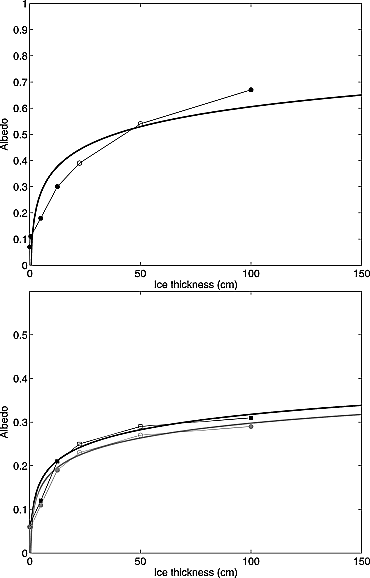
\includegraphics[trim=0cm 0cm 0cm 0cm,clip,width=8cm]{science/jgrd14967-fig-0001.png}
\fi
\]
\caption[Sea ice albedo as a function of ice thickness]{Sea ice albedo as a function of ice thickness for (top)
  visible (VIS, $\lambda < 689\,{\rm nm}$) and (bottom) near--infrared
(NIR, $\lambda > 689\,{\rm nm}$) spectral bands after
\cite{brandt2005}. The filled symbols are measurements, while the open
are interpolated values. The depths are the mean squares fit of the
form $\alpha_{\rm i}=a\log(h_{\rm i})+b$, where $a$ and $b$ are given
in Tab.~\ref{tab_bareseaice}. A distinction is made between direct
(black) and diffuse (gray) irradiance for NIR in
Fig.~\ref{fig_seaicealbedo} (bottom). Reprinted by permission from John
Wiley and Sons. Copyright 2009 by the American Geophysical Union.}\label{fig_seaicealbedo}
\end{figure}

\begin{table}
\caption[Constants for bare sea ice albedo]{Constants for bare sea ice albedo$^\ast$}\label{tab_bareseaice}
\begin{tabular*}{\textwidth}{l@{\extracolsep\fill}llc}\hline
& \multicolumn{1}{c}{$a$} & \multicolumn{1}{c}{$b$} & \multicolumn{1}{c}{Upper threshold} \\\hline
VIS & 0.13 & 0.10 & 0.76 \\
NIR direct & 0.047 & 0.074 & 0.29 \\
NIR diffuse & 0.049 & 0.085 & 0.31 \\\hline
\end{tabular*}
$^\ast$ Bare sea ice albedo is of the form $\alpha_{\rm
  i}=a\log(h_{\rm i}) + b$ proposed from data from \cite{brandt2005}
for visible (VIS, $\lambda < 689 \, {\rm nm}$) and near--infrared
(NIR, $\lambda > 689 \, {\rm nm}$) (direct and diffuse). The upper
threshold values are used for ice thicknesses equal to or above
$1.6\,{\rm m}$ for VIS and $1.0\,{\rm m}$ for NIR.
\end{table}

\subsubsection{Melt ponds}\label{sec_meltpond}

The inclusion of melt ponds in the albedo scheme is very important
from a physical perspective, because of their extensive presence
during summer \cite{perovich2002, tschudi2001, fetterer1998, perovich1997}, and
the large portion of solar energy absorbed by the melt water
(\cite{podgorny1996}). 
Both \cite{schramm1997} and \cite{morassutti1996} provide useful melt pond
albedo parameterizations as a function of pond depth. However, such
schemes cannot be used directly because melt pond depth, and also the
more important melt pond fraction (see
equation~(\ref{eq_seaicealbedo})), is not available in GCMs.

We propose a basic model for melt pond evolution based on the daily
surface ice melt rate from \echam. The temporal evolution of a melt
pond is calculated from the mass balance equation

\begin{equation}\label{eq_massbalance}
\frac{\partial p_{\rm d}}{\partial t} = -\frac{\rho_{\rm i}}{\rho_{\rm
    w}}
\left(\frac{\partial h_{\rm i}}{\partial t}+\frac{\partial p_{\rm
    di}}{\partial t}\right)-\left(\frac{\partial p_{\rm d}}{\partial
  t}\right)_s,
\end{equation}

where $p_{\rm d}$ is the pond depth in m and $\rho_{\rm w}$, $\rho_{\rm
  i}$ are the densities of water and ice, respectively
(Fig.~\ref{fig2}). The first term on the right hand side represents the
melt pond growth through the surface melting of sea ice; the second
term refers to the growth or melting of pond ice $p_{\rm di}$; and the
last term is the constant seepage rate. Pond ice forms if the
temperature of the pond, $T_{\rm w}$, falls below the freezing point,
$T_0$, where $T_{\rm w}$ is calculated from the heat budget equation

\begin{equation}
C_{\rm w}\frac{\partial T_{\rm w}}{\partial t}=H_{\rm sfc}.
\end{equation}

$C_{\rm w}$ is the heat capacity of the pond and $H_{\rm sfc}$ is the
sum of all radiative and turbulent heat fluxes at the surface of the
ice--free pond. For $T_{\rm w} < T_0$, a slab of ice is formed
according to 

\begin{equation}
p_{\rm di} = \left(\frac{C_{\rm w}}{L_{\rm f}\rho_{\rm
      i}}\right)(T_0-T_{\rm w}),
\end{equation}

where $L_{\rm f}$ is the latent heat of fusion. $T_{\rm w}$ is then
reset to $T_0$ and is kept fixed, independent of the sign of $H_{\rm
  sfc}$, because the pond water is forming on top of the ice. The
surface temperature of the ice, $T_{\rm i}$, is calculated from the
heat budget of a thin slab of ice (1~cm) at the surface

\begin{equation}
C_{\rm i}\frac{\partial T_{\rm i}}{\partial t}=H_{\rm sfc}+H_{\rm c},
\end{equation}

where $C_i$ is the heat capacity of the thin upper slab of pond ice
and $H_{\rm c}$ is the conductive heat flux through the ice given by

\begin{equation}\label{eq_condheatflux}
H_{\rm c}=\frac{\kappa_{\rm i}}{p_{\rm di}}(T_0-T_{\rm i})\ge 0,
\end{equation}

where $\kappa_{\rm i}$ is the thermal conductivity of ice.

\begin{figure}[htb]
\[
\ifpdf
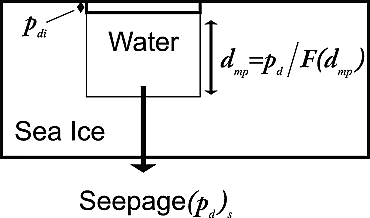
\includegraphics[trim=0cm 0cm 0cm 0cm,clip,width=8cm]{science/jgrd14967-fig-0002.png}
\fi
\]
\caption[A schematic drawing of a melt pond]{A schematic drawing of a melt pond describing a few of the
  variables in
  equations~(\ref{eq_massbalance})--(\ref{eq_condheatflux}). Reprinted by permission from John
Wiley and Sons. Copyright 2009 by the American Geophysical Union.}\label{fig2}
\end{figure}

Melt pond formation will not start before the snow on top of the sea
ice has melted away. If a slab of pond ice $p_{\rm di}\ge 1\,{\rm cm}$
is forming, the melt pond fraction is set to zero. The final closing
of the melt pond in fall is generally caused by vanishing melting and
constant seepage, resulting in $p_{\rm d} \le 0$, or by freezing if
the pond is totally frozen or if a thick ice layer has been formed
($p_{\rm di}=10\,{\rm cm}$). In all these cases the pond is closed,
i.e., $p_{\rm d}$ is set to zero.

To provide an estimate of the melt pond fraction, we propose to
calculate it from the melt pond depth (similar to what is done for
the snow cover fraction in GCMs) using a parameterization of the
results from a number of simulations using a small--scale melt pond
model (\cite{luethje2006}). The model treats the ice surface as a
porous medium. Melt water drains through the ice to the ocean at a
constant rate ($0.8\,{\rm cm/d}$) and the melt water left on the
surface percolates to lower lying areas to form melt ponds. The melt
rate is kept constant during the melt season, but is enhanced where
melt ponds form, to simulate the lower albedo of the melt ponds.
The model discretizes the space and time domain using a finite
differences scheme. For relating the melt pond depth and fraction
covered for different climate scenarios, the model was run with the
same input parameters as described in details by \cite{luethje2006} in
the study of \cite{pedersen2009}. The
melt rate for the ice surface was varied from $1.0\,{\rm cm/d}$ to
$3.0\,{\rm cm/d}$ (in steps of $0.1\,{\rm cm/d}$), while the enhanced
melt rate under the melt ponds was kept at twice the ice surface melt
rate. This was done for both a MYI and a FYI setting, resulting in a
total of 42~model runs, with a melt season of 71~days. The mean daily
fraction of the surface covered by melt ponds is plotted against the
daily mean melt pond depth in Fig.~\ref{fig3} (for FYI and MYI separately).

\begin{figure}[htb]
\[
\ifpdf
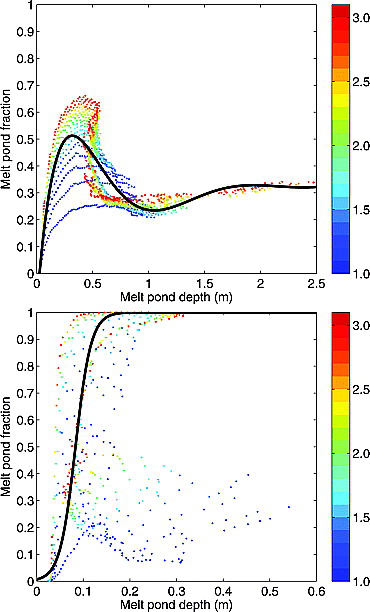
\includegraphics[trim=0cm 0cm 0cm 0cm,clip,width=8cm]{science/jgrd14967-fig-0003.png}
\fi
\]
\caption[Melt pond depth versus meltpond fraction]{Melt pond depth versus meltpond fraction for (top) multiyear
  ice (MYI) and (bottom) first year ice (FYI). The thick lines
  represent the best fit to the data. For MYI the best fit is
  represented by a 8--degree polynomial (equation(\ref{eq_polynom})),
  and for TYI it is represented by a hyperbolic tangent (equation
  (\ref{eq_tanh})). The scatter plot is based on the melt pond model
  by \cite{luethje2006} by using melt rates ranging from $1\,{\rm
    cm/d}$ to $3\,{\rm cm/d}$ (in steps of $0.1\,{\rm cm/d}$) as
  indicated by the color bar. Reprinted by permission from John
Wiley and Sons. Copyright 2009 by the American Geophysical Union.}\label{fig3}
\end{figure}

To connect the melt pond fraction to the melt pond depth for MYI
(Fig.~3, top), an 8--degree polynomial was fitted to the data points:

\begin{equation}\label{eq_polynom}
f_{\rm mp}= a d^8_{\rm mp}+b d^7_{\rm mp}+ c d^6_{\rm mp}+ d d^5_{\rm
  mp}+ e d^4_{\rm mp}+ f d^3_{\rm mp}+ g d^2_{\rm mp}+ h d_{\rm mp}+ i
\end{equation}

where $d_{\rm mp}$ is th melt pond depth in m, and the constants $a$
to $i$ are given in Tab.~\ref{tab_meltpondfit}.
\begin{table}[tb]
\begin{scriptsize}
\caption{Constants for melt pond fraction as a function of melt pond
  depth for multiyear ice}\label{tab_meltpondfit}
\begin{tabular*}{\textwidth}{c@{\extracolsep\fill}cccccccc}\hline
a & b & c & d & e & f & g & h & i\\\hline
-0.00724636 & 0.14438 & -1.19140 & 5.25995 & -13.37101 & 19.53030 &
-15.27019 & 5.26674 & -0.12549 \\\hline
\end{tabular*}
\end{scriptsize}
\end{table}
Fig.~\ref{fig3} (top) shows melt pond depths up to $2.5\,{\rm m}$ for
unrealistically high melt rates ($2.5-3.0\,~{\rm cm/d}$) during the
end of the 71 simulated days. Such depths are not realistic, and were
only included to avoid reaching outside the range of possible melt
pond depth. For FYI, the connection between fraction and depth is more
complex (Fig.~\ref{fig3}, bottom). For small melt rates, the
relationship is similar to that for MYI, but for more realistic melt
rates, the relationship is better described by a hyperbolic tangent
function,

\begin{equation}\label{eq_tanh}
f_{\rm mp}=0.5 \tanh(30 d_{\rm mp} - 2.5) + 0.5.
\end{equation}

Since melt ponds on FYI are mostly important in the beginning and
middle of the melt season, before the ice breaks up, the fit is
created to correspond best with this data, and less with the model
data from later in the melt season.

Regression equations were used for calculating the melt pond albedo
from melt pond depth from observations of melt pond albedo in the
Canadian Arctic Archipelago in spring and summer by~\cite{morassutti1996}:

\begin{equation}
\alpha_{\rm mp}=a+\exp(-b d_{\rm mp}-c)
\end{equation}

where $a$, $b$, and $c$ are regression coefficients, determined for
VIS ($400-689\,{\rm nm}$) and NIR ($689-1000\,{\rm nm}$) bands under
different light conditions (Tab.~\ref{tab_constmelt}). The exponential
albedo decay is large for the first $10-20\,{\rm cm}$ of pond depth,
and for deeper melt ponds the albedo is relatively constant.
An overview of the impact of melt ponds on Arctic sea ice is given in
the model study of \cite{roeckner2012}.
\begin{table}
\caption[Constants for melt pond albedo]{Constants for melt pond albedo$^\ast$}\label{tab_constmelt}
\begin{tabular*}{\textwidth}{l@{\extracolsep\fill}ccc}\hline
 & $a$ & $b$ & $c$ \\\hline
VIS direct & 0.336 & \cw{0}9.457 & 1.061 \\
VIS diffuse & 0.413 & 24.014 & 1.086 \\
NIR direct & 0.017 & 18.904 & 0.909 \\
NIR diffuse & 0.061 & 17.449 & 1.075 \\\hline
\end{tabular*}
$^\ast$Melt pond albedo $\alpha_{\rm mp}$ is of the form $\alpha_{\rm
  mp}=a+\exp(-b d_{\rm mp} - c)$ as a function of melt pond depth
$d_{\rm mp}$ from~\cite{morassutti1996} for visible (VIS) and
near--infrared (NIR) and direct and diffuse radiation.
\end{table}
